\documentclass[]{scrartcl}

\usepackage {listings}
\usepackage[ngerman]{babel}
\usepackage[utf8]{inputenc}
\usepackage{graphicx}
\usepackage{xcolor}
\usepackage{hyperref}

\setlength{\parindent}{0em}


%opening
\title{Räuber-Beute-Simulation}
\subtitle{Zellularautomaten - SL1 - Soft Computing - SS17}
\author{Benedikt Straube}

\begin{document}

\maketitle

\newpage

\section{Installation}
Zur lokalen Ausführung der Applikation ist eine NodeJs Installation notwendig. Diese sollte mindestens in Version 6.11.0 (\url{https://nodejs.org/}) zur Verfügung stehen.

Im nächsten Schritt sollten innerhalb des Projektverzeichnisses die notwendigen Pakete für eine lokale Ausführung installiert werden. Dies ist möglich via 
\begin{lstlisting}[backgroundcolor=\color{lightgray}]
npm install
\end{lstlisting}

Nachdem alle notwendigen Pakete installiert wurden, kann ein lokaler Server mittels
\begin{lstlisting}[backgroundcolor=\color{lightgray}]
npm start
\end{lstlisting}
gestartet werden.

Danach ist die Applikation im Browser über \url{http:localhost:4200} zu erreichen.

\newpage
\section{Ausführung}
\label{ausfuehrung}
Die Applikation kann über die beschriebe Installation lokal gestartet und über den Browser bedient werden. Weiterhin wird der compilierte Code zusätzlich über GitHub-Pages gehostet. Dadurch ist die Applikation auch unter der URL \url{https://benediktst.github.io/Soft-Computing-VAWI} zu erreichen.

Vorsicht: Hier existiert zum aktuellen Zeitpunkt noch ein Bug des Routings, was bei dem Refresh der Applikation zu einer 404-Seite führt. Die Applikation kann immer wieder über die Angegebene URL erreicht werden.

\begin{figure}[htbp]
	\centering
	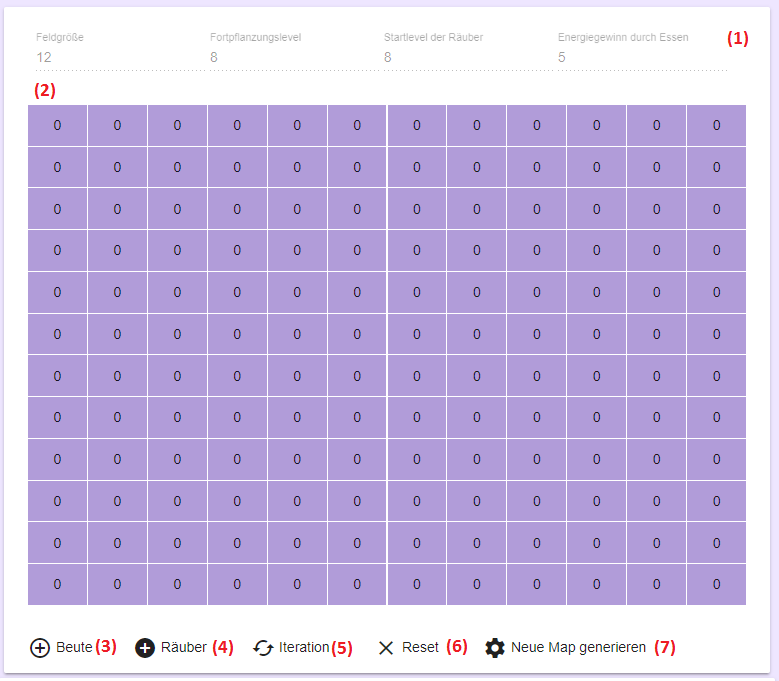
\includegraphics[width=0.8\textwidth]{res/interface.png}
	\caption{Aktionsmöglichkeiten der Anwendung}
	\label{img:interface}
\end{figure}

Um die Implementierung der SL-1 zu erreichen muss innerhalb der Kopfzeile ganz rechts das Menü geöffnet und die Option SL-1 ausgewählt werden. In der Anwendung (siehe Abbildung \ref{img:interface}) können an erster Stelle (1) die Einstellungen der Karte entnommen werden. Unter (2) ist die Karte mit allen Zellen dargestellt. Per Klick in eine Zelle kann das Detail-Menü zu dieser Zelle geöffnet werden. Durch (3) wird eine Beute auf einem zufälligen Feld hinzugefügt und unter (4) entsprechend ein Räuber. Mittels (5) wird durch den Prozess iteriert und es wird immer eine Kalkulation aller Zellen ausgeführt. (6) Setzt den Status der Zellen zurück auf den Ausgangszustand. (7) Öffnet die Eingabemaske um eine neue Map/Karte zu generieren.\\

\begin{figure}[htbp]
	\centering
	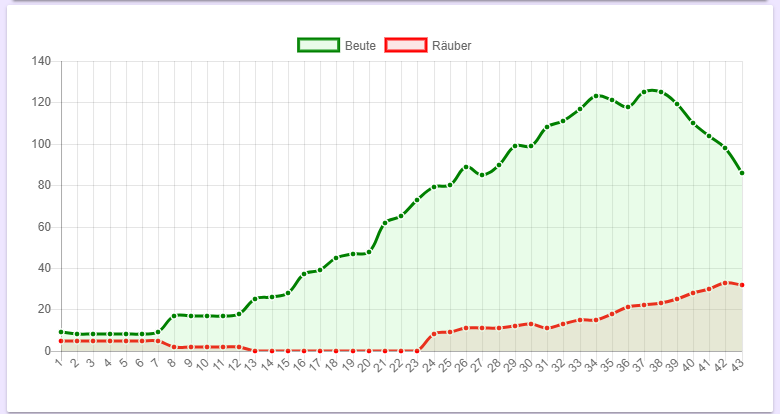
\includegraphics[width=0.8\textwidth]{res/graph.png}
	\caption{Visualisierung des Räuber-Beute-Verhältnisses}
	\label{img:graph}
\end{figure}

Zusätzlich zu der Karte werden die Summen der Räuber und der Beute in einem Grafen (Abbildung \ref{img:graph}) mitprotokolliert, um dort einen Verlauf des Geschehens entnehmen zu können

\newpage
\section{Logik des unterliegenden Systems}
\label{logik}
Das System soll das Verhalten von Räubern und deren Beute in einem abgeschlossenen Raum betrachten. Dabei sind die Kernbestandteile Fortpflanzung, Bewegung und Fressen. Die Zellen sind mit folgenden Eigenschaften umgesetzt:
\begin{itemize}
	\item Koordinaten zur Bestimmung der Position
	\item Einen Wert, welcher das Level, die Fitness bzw. das Alter der Zelle ausdrückt. Dieses Level wird für die Fortpflanzung und Ernährung verwendet
	\item Eine ID, um belegte Zellen eindeutig zu identifizieren und eine Bewegung über mehrere Stufen zu ermöglichen
	\item Einen Typen, welcher ausdrückt, ob es sich um einen Räuber, eine Beute oder ein Leeres Feld handelt
	\item Und eine Farbe für die Darstellung der Typen im UI
	\item Eine Ausrichtung, welche die Bewegungsabsicht darstellt
	\item Eine Marke, ob sich die Zelle Fortgepflanzt hat.
\end{itemize}

\subsection{Regeln}
\label{rules}
Für die Zellen werden entsprechende Regeln hinterlegt, dabei gelten alle Regeln für jede Zelle. Innerhalb er Regeln können dann allerdings Filter für beispielsweise nur Räuber angewendet werden. Folgende Regeln wurden implementiert:
\begin{itemize}
	\item Eine Zelle vom Typ Beute erhöht jede Iteration ihr Level, außer sie war Teil einer Fortpflanzung.
	\item Eine Zelle vom Typ Räuber vermindert jede Iteration ihr Level.
	\item Eine Zelle wird gelöscht, wenn ihr Level \(<=0\) fällt.
	\item Eine Zelle vom Typ Beute wird für die nächste Iteration nicht mehr als Teil der Fortpflanzung betrachtet.
	\item Eine Zelle vom Typ Beute erhöht erzeugt eine neue Zelle vom Typ Beute mit dem Level=1, wenn ihr eigenes Level das notwendige PopulationsLevel erreicht hat und der ausreichende Platz dafür vorhanden ist. Ihr Level wird dabei halbiert.
	\item Eine Zelle vom Typ Beute entscheidet, in welche Richtung sie sich bewegen möchte. Dies passiert zufällig und kann nur auf freie Felder geschehen. In dieser Regel findet noch keine Bewegung statt, sondern nur die Bestimmung der Richtung.
	\item Eine Zelle vom Typ Räuber entscheidet, in welche Richtung sie sich bewegen möchte. Der Räuber bewegt sich auf das Feld einer Beute zu. Wenn keine Beute im Umkreis ist, bewegt sich der Räuber auf ein zufälliges Feld.
	\item Eine Zelle vom Typ Beute setzt die bereits definierte Bewegung um. Dies basiert auf der Ausrichtung der Zelle. Die Ausgangszelle wird bei diesem Schritt geleert.
	\item Eine Zelle vom Typ Räuber setzt die bereits definierte Bewegung um. Dies basiert auf der Ausrichtung der Zelle. Falls die neue Zelle eine Beute ist, wird diese entfernt. Die Ausgangszelle wird bei diesem Schritt geleert.
\end{itemize}

\subsection{Reihenfolge der Regeln}
\label{reihenfolge}
Aufgrund der Bewegung war es notwendig manche Regeln sequenziell nach anderen Ablaufen zu lassen, um eine Konsistenz zu gewährleisten. Im ersten Schritt werden für alle Felder die Aktivitäten zum Fortpflanzen, Energiegewinn, Energieverlust, die Bewegungsrichtung verarbeitetet. Danach werden alle werden für alle Felder, welche vom Typ Räuber sind die Bewegung der Räuber durchgeführt. Direkt im Anschluss für alle leeren Felder. Dies sorgt für einen konsistenten Stand da die Räuber quasi kurzzeitig dupliziert und wieder aufgeräumt wurden. Dieses Schema wird danach auch für die Beute verwendet. Zum Schluss werden Zellen mit einem zu niedrigen Level gelöscht und der Fortpflanzungsstatus bei allen Zellen zurückgesetzt

\newpage
\section{Aufbau der Applikation}
\label{aufbau}
Das Framework zur Implementierung ist Angular. Es nimmt keine bedeutenden Eingriffe in die Implementierung der Logik, sondern übernimmt hauptsächlich die Darstellung innerhalb des Browsers.


Die Implementierung erfolgt innerhalb nachfolgender Orderstruktur:
\begin{lstlisting}[backgroundcolor=\color{lightgray}]
src
|- app
   |- predator-prey
\end{lstlisting}
Außenstehende Komponenten sind zur Navigation und Verwaltung notwendig.

Innerhalb des EA-Ordners befinden sich folgende Dateien:
\begin{itemize}
\item predator-prey.component.css (Styling der Komponente)
\item predator-prey.component.html (Strukturierung der Komponente)
\item predator-prey.component.ts (Logik der Komponente)
\end{itemize}

Im util-Ordner stehen noch weitere Klassen zur Verfügung, auf welche im Folgenden genauer eingegangen werden soll.
\begin{itemize}
	\item cell.ts (Modell einer Zelle)
	\item map.ts (Implementierung der Karte einschließlich Regelablauf)
	\item rules.ts (Alle beschriebenen Regeln)
\end{itemize}

Die \textit{Cell}-Klasse enthält all die Informationen welche in Kapitel \ref{logik} definiert werden. Zusätzlich ist dort noch ein Enum für die Verwaltung der Ausrichtung der Zelle hinterlegt. Interessant ist hier, dass diese Zellen keine weitere Funktion benötigen. Sie besitzen von sich aus keine Intelligenz oder Funktionalitäten, sondern werden nur durch eine Externe Betrachtung in Kombination mit ihrer Umgebung verändert.

Die \textit{Map}-Klasse enthält als wichtigstes Attribut ein zweidimensionales Array an Zellen. Die Map enthält die Möglichkeit die Zellen basierend auf deren Koordinaten auszugeben oder zu setzen. Es können mittels der \textit{getNeighbours}-Methode die direkten Nachbarzellen zu einer Zelle ermittelt werden. Per \textit{addPrey}- oder \textit{addPredator} können die entsprechenden Zellen entweder an einer übergebenen Position oder zufällig auf ein freies Feld hinzugefügt werden. Zuletzt ist hier noch die \textit{iterate}-Methode implementiert, welche die Reihenfolge der Regelanwendung nach Kapitel \ref{reihenfolge} umsetzt.

Die \textit{Rule}-Klasse enthält alle in Kapitel \ref{rules} definierten Regeln. Alle Regeln sind hier nach einem einheitlichen Design aufgebaut. Sie erhalten immer eine Referenz auf die Nachbarn der betrachteten Zelle und die betrachtete Zelle an sich als Übergabeparameter. Als Ergebnis wird immer eine Zelle zurückgegeben. Falls die Regel in einem Fall nichts verändern sollte, so wird die betrachtete Eingangszelle einfach zurückgegeben.

Die \textit{Predator-Prey}-Komponente besitzt hier keine eigene Logik sondern leitet lediglich die Eingaben über das UI an die entsprechenden Komponenten weiter. 


\newpage
\section{Ergebnisse}
\label{ergebnisse}

\subsection{Fehleranalyse in dem System}
Bei der Implementierung und besonders bei der Analyse der Ergebnisse ist hier aufgefallen, dass sich derartig entworfene Systeme extrem schwer Analysieren und Debuggen lassen. Bei vielen Zellen lassen sich die Zustände vor allem während den Regeln sehr schwer ermitteln und dann richtig interpretieren. Das hat auch dazu geführt, dass sich in der aktuellen Implementierung noch ein Bug befindet, welcher Räuber unter unklaren Umständen Reproduziert. Durch die schlechte Analysierbarkeit konnte dieser vor der Abgabe nicht mehr entfernt werden.

\subsection{Bewegung von Zellen}
Die Umsetzung von Bewegung der einzelnen Zellen hat zu weiteren Problemen geführt und den zuvor beschriebenen Aspekt verstärkt. Es wurde sich dann für eine sequentielle Abarbeitung der Bewegungs-regeln entschieden, wie in Kapitel \ref{reihenfolge} dargestellt wurde. Dennoch erscheint diese Lösung nicht ganz sauber, da sich das gesamte System bei dieser Umsetzung zwischenzeitlich in einem Inkonsistenten Stand befindet. Durch die Begrenzung auf die direkten Nachbarn war es aber mit einer anderen Implementierung nicht vermeidbar, dass sich zwei Zellen, welche nicht in direkter Nachbarschaft, sondern in einer einfach erweiterten Nachbarschaft zueinander sind, nicht die Bewegung auf das gleiche Feld durchführen. 


\subsection{Einfluss der Feldgröße}
Trotz einem Fehler in der Implementierung ist deutlich erkennbar, dass die Feldgröße einen starken Einfluss auf das Ergebnis und das Verhältnis zwischen Räuber und Beute hat. Kleine Felder sind eindeutig ein Vorteil für Räuber, da sie hier schnell entsprechende Beute finden und meist von dort an immer weiter Fressen können. Bei Großen Feldern hingegen ist es nicht unüblich, dass bereits einige Räuber aussterben, bevor sie in der nähe eines Beutetieres waren. Daher sind die Faktoren Feldgröße und Dichte der belegten Felder eindeutig sehr relevant für das Ergebnis.


\end{document}
